\documentclass[12pt]{article}
\usepackage[spanish]{babel}
\usepackage{geometry}
\geometry{a4paper, margin=1in}
\usepackage{graphicx}
\usepackage{xcolor}
\usepackage{titlesec}
\usepackage{parskip}
\usepackage{multicol}
\usepackage{cite}
\usepackage{listings}
\usepackage{color}
\usepackage{amsmath}
\usepackage{enumitem}

\lstset{
  language=Python,
  basicstyle=\ttfamily\small,
  keywordstyle=\color{blue},
  commentstyle=\color{gray},
  stringstyle=\color{red},
  breaklines=true,
  showstringspaces=false
}


\definecolor{highlight}{RGB}{255, 255, 0}

\titleformat{\section}{\normalfont\Large\bfseries}{\thesection}{1em}{}
\titleformat{\subsection}{\normalfont\large\bfseries}{\thesubsection}{1em}{}

\begin{document}

% Logos
\begin{minipage}{0.45\textwidth}
    
\includegraphics[width=0.4\textwidth]{inFiles/Figures/epnLogo.jpg}
\end{minipage}
\hfill
\begin{minipage}{0.45\textwidth}
    \raggedleft
    
\includegraphics[width=0.4\textwidth]{inFiles/Figures/FIS_logo.jpg}
\end{minipage}

\vspace{0.5cm}

% Títulos principales
\begin{center}
    \textbf{ESCUELA POLITÉCNICA NACIONAL}\\[0.2cm]
    \textbf{FACULTAD DE INGENIERÍA DE SISTEMAS}\\[0.2cm]
    \textbf{INGENIERÍA EN CIENCIAS DE LA COMPUTACIÓN}
\end{center}

\vspace{0.5cm}
\hrule
\vspace{0.5cm}

% Datos principales
\noindent\textbf{PERÍODO ACADÉMICO:} 2025-A\\[0.2cm]
\noindent\textbf{ASIGNATURA:} ICCD412 Métodos Numéricos \hfill \textbf{GRUPO:} GR2\\[0.2cm]
\noindent\textbf{TIPO DE INSTRUMENTO:} Práctica3\\[0.2cm]
\noindent\textbf{FECHA DE ENTREGA LÍMITE:} {07/05/2025}\\[0.2cm]
\noindent\textbf{ALUMNO:} {Sebastián Chicaiza}

\vspace{0.5cm}
\hrule
\vspace{1cm}


% Secciones
\section*{TEMA}

\begin{center}
    \Large\textbf{Método de la bisección}
\end{center}
\vspace{0.5cm}

\section*{OBJETIVOS}
\begin{itemize}
    \item {Conocer como aplicar el método de la bisección para sacar soluciones aproximadas a ecuaciones no lineales.}
    \item {Analizar el comportamiento y la presición del método de la bisección.}
\end{itemize}
\vspace{0.5cm}
\section*{MARCO TEÓRICO}
El método de la bisección es un proceso iterativo que consiste en evaluar una funcion \(f(x)\) en el punto medio \(p\) de un intervalo de interés \((x_1,x_2)\).
Dependiendo si su ordenada tiene el mismo signo que \(f(p)\) o no, se definirá que punto limite del intervalo tomará el valor \(p\) en la siguiente iteración. 
Este proceso se repetirá hasta que el intervalo esté dentro de un rango aceptable de error, es decir menor que una toleracia prefijada\cite{mathews2000metodos}.

Para aplicar el método de la bisección se utilizan los siguientes teoremas:

\textbf{Teorema del valor intermedio}

Si \(f \in C[a,b]\) y \(K\) es cualquier número entre \(f(a)\) y \(f(b)\), entonces existe un número \(c\) en \((a,b)\) para el cual \(f(c) = K\).

\textbf{Búsqueda de cambio de signo}

Un intervalo \([a,b]\), la función \(f(x)\) toma valores de diferente signo en los extremos.
\[f(a) \cdot f(b) < 0\]

\section*{DESARROLLO}

\subsection*{Ejercicios Aplicados}

\begin{enumerate}
    \item Un abrevadero de longitud \(L\) tiene una sección transversal en forma de semicírculo con radio \(r\). (Consulte la
    figura adjunta.) Cuando se llena con agua hasta una distancia \(h\) a partir de la parte superior, el volumen \(V\) de
    agua es
    \[V = L \left[ 0.5\pi r^{2} - r^{2}\arcsen{\left( \frac{h}{r} \right)} - h(r^{2} - h^{2})^{1/2} \right]\]
    \begin{center}
        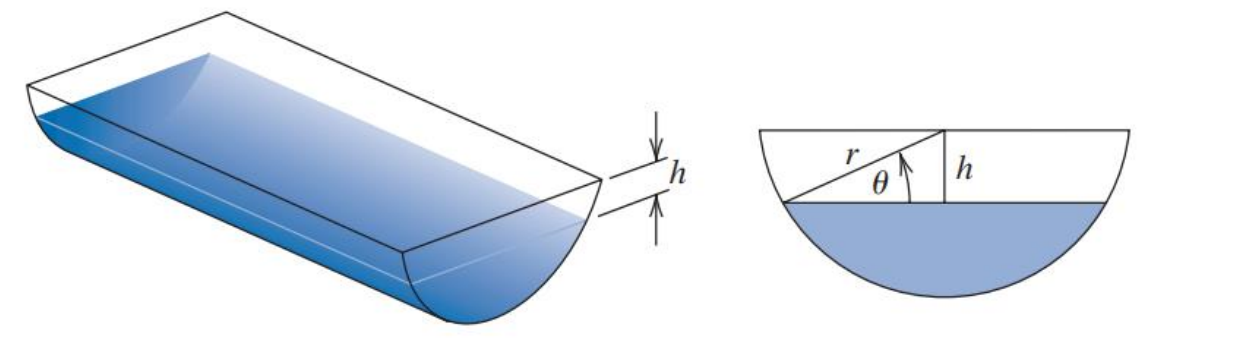
\includegraphics[width=0.9\textwidth]{inFiles/Figures/ej1Biseccion.png} 
    \end{center}

    Suponga que \(L = 10 cm\), \(r = 1 cm \) y \(V = 12.4 cm^{3}\). Encuentre la profundidad del agua en el abrevadero dentro de \(0.01 cm\).

    \[L \left[ 0.5\pi r^{2} - r^{2}\arcsen{\left( \frac{h}{r} \right)} - h(r^{2} - h^{2})^{1/2} \right] - V = 0\]
    \[ 10 \left[ 0.5\pi 1^{2} - 1^{2}\arcsen{\left( \frac{h}{1} \right)} - h(1^{2} - h^{2})^{1/2} \right] - 12.4 = 0 \]
    
    Usando el método de bisección, con una tolerancia de \(10^{-2}\) y un redondeo a 6 cifras significativas:

    \begin{center}
        \begin{tabular}{|c|c|c|c|c|c|c|}
        \hline
        \textbf{a} & \textbf{b} & \textbf{p} & \textbf{f(a)}&\textbf{f(b)}&\textbf{f(p)} &  \textbf{TOL} \\ \hline
        0.0 & 1.0 & 0.5 & 3.307963 & -12.4 & 2.402103 & 0.5 \\
        0.5 & 1.0 & 0.75 & 2.402103 & -12.4 & -0.211874 & 0.25 \\
        0.5 & 0.75 & 0.625 & 2.402103 & -0.211874 & 1.435553 & 0.125 \\
        0.625 & 0.75 & 0.6875 & 1.435553 & -0.211874 & 0.720073 & 0.0625 \\
        0.6875 & 0.75 & 0.71875 & 0.720073 & -0.211874 & 0.285179 & 0.03125 \\
        0.71875 & 0.75 & 0.734375 & 0.285179 & -0.211874 & 0.045035 & 0.015625 \\
        0.734375 & 0.75 & 0.742188 & 0.045035 & -0.211874 & -0.081246 & 0.007812 \\
        \hline
        \end{tabular}
    \end{center}
    
    La raiz aproximada de la función
    
    \[ f(h) = 10 \left[ 0.5\pi 1^{2} - 1^{2}\arcsen{\left( \frac{h}{1} \right)} - h(1^{2} - h^{2})^{1/2} \right] - 12.4 ,\]
    
    es \(h \approx 0.734375 \, cm\)

    \item Un objeto que cae verticalmente a través del aire está sujeto a una resistencia viscosa, así como a la fuerza
    de gravedad. Suponga que un objeto con masa \(m\) cae desde una altura \(s_0\) y que la altura del objeto después
    de \(t\) segundos es
    \[s(t) = s_0 - \frac{mg}{k}t + \frac{m^{2}g}{k^{2}} \left( 1- e^{-kt/m}\right),\]
    donde \(g = 9.81\, m/s^{2}\) y \(k\) representa el coeficiente de la resistencia del aire en \(\frac{Ns}{m}\). Suponga \(s_0 = 300\, m\),
    \(m = 0.25\, kg\) y \(k = 0.1 \frac{Ns}{m}\). Encuentre, dentro de \(0.01\, segundos\), el tiempo que tarda un cuarto de \(kg\) en golpear el piso. 
    
    Interesa saber \(t\) cuando \(s(t) = 0\)
    \[s(t) = s_0 - \frac{mg}{k}t + \frac{m^{2}g}{k^{2}} \left( 1- e^{-kt/m}\right) = 0\]
    \[300 - \frac{0.25 \cdot 9.81}{0.1}t + \frac{0.25^{2} \cdot 9.81}{0.1^{2}} \left( 1 - e^{-0.1t/0.25}\right) = 0\]

    Usando el método de bisección para encontrar la raíz de la funcion \(s(t)\) con una tolerancia de \(10^{-2}\):
    \begin{center}
        \begin{tabular}{|c|c|c|c|c|c|c|}
        \hline
        \textbf{a} & \textbf{b} & \textbf{p} & \textbf{s(a)}&\textbf{s(b)}&\textbf{s(p)} &  \textbf{TOL} \\ \hline
        0.0 & 25.0 & 12.5 & 300.0 & -251.815284 & 54.33688 & 12.5 \\
        12.5 & 25.0 & 18.75 & 54.33688 & -251.815284 & -98.565161 & 6.25 \\
        12.5 & 18.75 & 15.625 & 54.33688 & -98.565161 & -22.008986 & 3.125 \\
        12.5 & 15.625 & 14.0625 & 54.33688 & -22.008986 & 16.20856 & 1.5625 \\
        14.0625 & 15.625 & 14.84375 & 16.20856 & -22.008986 & -2.892249 & 0.78125 \\
        14.0625 & 14.84375 & 14.453125 & 16.20856 & -2.892249 & 6.660469 & 0.390625 \\
        14.453125 & 14.84375 & 14.648438 & 6.660469 & -2.892249 & 1.884632 & 0.195312 \\
        14.648438 & 14.84375 & 14.746094 & 1.884632 & -2.892249 & -0.50368 & 0.097656 \\
        14.648438 & 14.746094 & 14.697266 & 1.884632 & -0.50368 & 0.690509 & 0.048828 \\
        14.697266 & 14.746094 & 14.72168 & 0.690509 & -0.50368 & 0.093422 & 0.024414 \\
        14.72168 & 14.746094 & 14.733887 & 0.093422 & -0.50368 & -0.205127 & 0.012207 \\
        14.72168 & 14.733887 & 14.727783 & 0.093422 & -0.205127 & -0.05584 & 0.006104 \\
        \hline
        \end{tabular}
    \end{center}

    El tiempo \(t\) que tarda el objeto en tocar el piso es \(t \approx 14.733887 \, segundos\) 
\end{enumerate}

\subsection*{Ejercicios Teóricos}

\begin{enumerate}       
    \item Use el teorema 2.1 para encontrar una cota para el número de iteraciones necesarias para lograr una
    aproximación con precisión de \(10^{-4}\) para la solución de \(x^{3} -x -1 = 0\) que se encuentra dentro del intervalo
    \([1, 2]\). Encuentre una aproximación para la raíz con este grado de precisión.
    \[ error_{abs} < 10^{-4}\quad \text{y} \quad error_{abs} \leq \frac{b-a}{2^{n}}\]
    entonces: 
    \[
        \begin{aligned}
            \frac{b-a}{2^{n}} &< 10^{-4} \\
            \frac{1}{2^{n}} &< 10^{-4} \\
            2^{-n} &< 10^{-4}\\
            \log_{2}{(2^{-n})} &<  \log_{2}{(10^{-4})}\\
            -n \cdot \log_{2}{(2)} &< -4 \cdot \log_{2}{(10)} \\
            n &> 4 \cdot \log_{2}{(10)} \\
            n &> 13.2876 \\
            n &\approx 14
        \end{aligned}
    \]

    Usando el método de bisección con una tolerancia de \(10^{-4}\) para la función \(f(x) = x^{3} -x -1\) con 14 intentos:
    
    \begin{center}
        \begin{tabular}{|c|c|c|c|c|c|c|}
        \hline
        \textbf{a} & \textbf{b} & \textbf{p} & \textbf{f(a)}&\textbf{f(b)}&\textbf{f(p)} &  \textbf{TOL} \\ \hline
        1.0 & 2.0 & 1.5 & -1.0 & 5.0 & 0.875 & 0.5 \\
        1.0 & 1.5 & 1.25 & -1.0 & 0.875 & -0.296875 & 0.25 \\
        1.25 & 1.5 & 1.375 & -0.296875 & 0.875 & 0.224609 & 0.125 \\
        1.25 & 1.375 & 1.3125 & -0.296875 & 0.224609 & -0.051514 & 0.0625 \\
        1.3125 & 1.375 & 1.34375 & -0.051514 & 0.224609 & 0.082611 & 0.03125 \\
        1.3125 & 1.34375 & 1.328125 & -0.051514 & 0.082611 & 0.014576 & 0.015625 \\
        1.3125 & 1.328125 & 1.320312 & -0.051514 & 0.014576 & -0.018713 & 0.007812 \\
        1.320312 & 1.328125 & 1.324218 & -0.018713 & 0.014576 & -0.002131 & 0.003907 \\
        1.324218 & 1.328125 & 1.326172 & -0.002131 & 0.014576 & 0.006209 & 0.001954 \\
        1.324218 & 1.326172 & 1.325195 & -0.002131 & 0.006209 & 0.002035 & 0.000977 \\
        1.324218 & 1.325195 & 1.324707 & -0.002131 & 0.002035 & -0.000047 & 0.000489 \\
        1.324707 & 1.325195 & 1.324951 & -0.000047 & 0.002035 & 0.000994 & 0.000244 \\
        1.324707 & 1.324951 & 1.324829 & -0.000047 & 0.000994 & 0.000474 & 0.000122 \\
        1.324707 & 1.324829 & 1.324768 & -0.000047 & 0.000474 & 0.000213 & 0.000061 \\
        \hline
        \end{tabular}

    \end{center}
    Raíz aproximada de \(f(x) = x^{3} -x -1\), dentro de la tolerancia \(10^{-4}\):
    
    \(x \approx 1.324829 \)

    \item La función definida por \(f(x) = \sin{\pi} x\) tiene ceros en cada entero. Muestre cuando \(-1 < a< 0\) y \(2 < b< 3\),
    el método de bisección converge a

    \begin{enumerate}[label=\alph*.]
        \item \(0, si \quad a+b<2\)
        \[ a = -0.75 \quad \text{y} \quad b = 2.25 \]
        \begin{tabular}{|c|c|c|c|c|c|c|}
            \hline
            \textbf{a} & \textbf{b} & \textbf{p} & \textbf{f(a)}&\textbf{f(b)}&\textbf{f(p)} &  \textbf{TOL} \\ \hline
            -0.75 & 2.25 & 0.75 & -0.707107 & 0.707107 & 0.707107 & 1.5 \\
            -0.75 & 0.75 & \textcolor{red}{0.0} & -0.707107 & 0.707107 & 0.0 & 0.75 \\
            \hline
            
        \end{tabular}
        \item \(2, si \quad a+b>2\)
        \[ a = -0.25\quad \text{y} \quad b = 2.75 \]
        \begin{tabular}{|c|c|c|c|c|c|c|}
            \hline
            \textbf{a} & \textbf{b} & \textbf{p} & \textbf{f(a)}&\textbf{f(b)}&\textbf{f(p)} &  \textbf{TOL} \\ \hline
            -0.25 & 2.75 & 1.25 & -0.707107 & 0.707107 & -0.707107 & 1.5 \\
            1.25 & 2.75 & \textcolor{red}{2.0} & -0.707107 & 0.707107 & -0.0 & 0.75 \\
            \hline
            
        \end{tabular}
        \item \(1, si \quad a+b=2\)
        \[ a = -0.5 \quad \text{y} \quad b = 2.5 \]
        \begin{tabular}{|c|c|c|c|c|c|c|}
            \hline
            \textbf{a} & \textbf{b} & \textbf{p} & \textbf{f(a)}&\textbf{f(b)}&\textbf{f(p)} &  \textbf{TOL} \\ \hline
            -0.5 & 2.5 & \textcolor{red}{1.0} & -1.0 & 1.0 & 0.0 & 1.5 \\
            \hline
            
        \end{tabular}
    \end{enumerate}
\end{enumerate}     
\section*{CONCLUSIONES}
\begin{itemize}
    \item {El método de bisección es una forma de encontrar raíces aproximadas de una función.}
    \item {El método de bisección es confiable ya que siempre converge.} 
\end{itemize}

\section*{RECOMENDACIONES}

Usar herramientas que nos permitan gráficar funciones, ya que se puede apreciar má facilmente si es que el método ha sido bien aplicado.
\renewcommand{\refname}{\MakeUppercase{REFERENCIAS}}
\bibliographystyle{IEEEtran}
\bibliography{inFiles/References/references.bib}


\end{document}
